%\clearpage
\section{Empirical Performance Analysis}\label{sec:experiments}
In this section, we perform an empirical evaluation of {\fairXplainer}. In the following, we discuss the experimental setup, the objectives of experiments, and experimental results. { We adjoin the source code and additional experimental results on the effects of maximum order $\lambda$, runtime, accuracy on different datasets and corresponding explanations (Appendix~\ref{sec:additional_experiments}) to the supplementary material.}

\noindent\textbf{Experimental Setup.} We implement a prototype of {\fairXplainer} in Python (version $ 3.8 $). In {\fairXplainer}, we deploy SAlib library~\cite{Herman2017} to compute FIFs leveraging techniques of global sensitivity analysis. In our experiments, we consider five widely studied datasets from fairness literature, namely COMPAS~\cite{angwin2016machine}, Adult~\cite{DK2017uci}, German-credit~\cite{DK2017}, Ricci~\cite{mcginley2010ricci}, and Titanic (\url{https://www.kaggle.com/c/titanic}). We deploy Scikit-learn~\cite{scikit-learn} to learn different classifiers: Logistic Regression, Support Vector Machine, Decision Tree, and Neural Networks. In experiments, we specify {\fairXplainer} to compute intersectional influences up to second order ($ \lambda = 2 $). We compare {\fairXplainer} with Shapley-valued based FIF computational framework, referred as SHAP~\cite{lundberg2020explaining}. In addition, we deploy {\fairXplainer} along with different fairness-enhancing~\cite{kamiran2012data} and fairness attack~\cite{solans2020poisoning} algorithms, and analyze the effect of these algorithms on the FIFs and the resultant fairness metric. In the following, we discuss the objective of our empirical study. 
\begin{enumerate}[nosep,leftmargin=*]
%\begin{enumerate}
	\item How do \textbf{accuracies} of {\fairXplainer} and SHAP compare for estimating FIFs and resulting bias?
	\item What is the impact of\textbf{ intersectional vs.\ individual FIFs} in tracing the sources of bias?
    \item How do FIFs change while \textbf{applying} different fairness enhancing algorithms, i.e. \textbf{affirmative actions}, and fairness attacks, i.e. \textbf{punitive actions}?
	%\item \red{What is the effect of $ \lambda $ on the runtime of {\fairXplainer}?}
\end{enumerate}
In summary, \textit{{\fairXplainer} achieves significantly less estimation error than SHAP in all the datasets.} This shows the importance of adopting global sensitivity analysis to compute FIFs for group fairness metrics than local explanation approaches. Moreover, \textit{{\fairXplainer} effectively traces the sources of bias by computing intersectional FIFs, which earlier method like SHAP {did not capture}.} {\fairXplainer} also detects the effects of the affirmative and punitive actions on the bias of a classifier and the corresponding tensions between different subsets of features. %Due to brevity of space, we defer additional experimental results to the Supplementary material. %In the following, we elaborate results on estimation error and individual vs.\ intersectional FIFs.




\begin{figure}[!t]
	\begin{minipage}{0.49\textwidth}
		\centering
		\subfloat[Statistical parity]{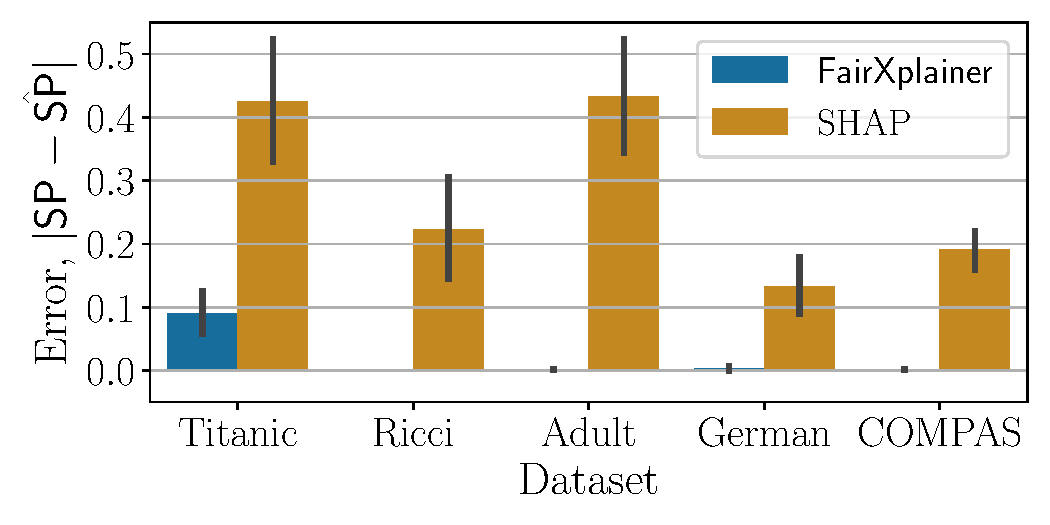
\includegraphics[scale=0.39]{figures/fairness/fif/sp_train_accuracy}}
	\end{minipage}
	\begin{minipage}{0.5\textwidth}
		\centering
		\subfloat[Equalized odds]{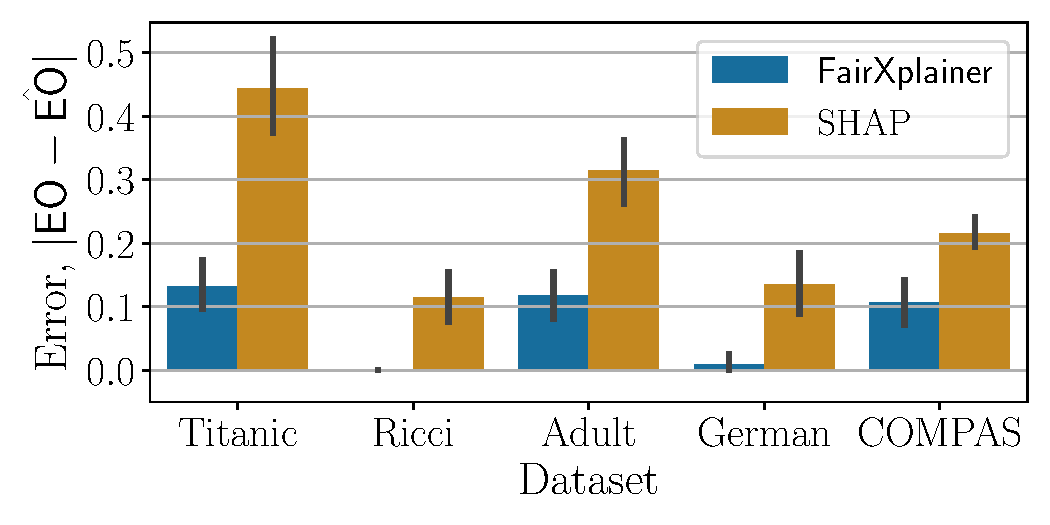
\includegraphics[scale=0.39]{figures/fairness/fif/eo_train_accuracy}}
	\end{minipage}
	\caption[Accuracy of {\fairXplainer}]{Comparing {\fairXplainer} and SHAP on the estimation error of fairness metrics. Lower values on the $ Y $-axis denote a better result. {\fairXplainer} has significantly less error than SHAP.}\label{fig:estimation_error}
%	\vspace{-0.5em}
\end{figure}
\noindent\textbf{Accurate Estimation of Bias.} We compare {\fairXplainer} with SHAP in estimating Statistical Parity $(\mathsf{SP})$ and Equalized Odds $(\mathsf{EO})$, where each metric is calculated by summing all FIFs (Axiom~\ref{axm:additivity}). We consider five datasets, each trained on different classifiers by applying five-fold cross-validation. We compute estimation error by taking the absolute difference between the exact and  estimated value of a metric, and present results in Figure~\ref{fig:estimation_error}. In both metrics, {\fairXplainer} demonstrates significantly less error than SHAP. For example, the mean error of {\fairXplainer} in estimating $ \mathsf{SP} $ on Titanic dataset is $ 0.1 $ vs.\ $ 0.42 $ for SHAP. In this context, the error of {\fairXplainer} is often zero in most datasets and only insignificant ($ \le 0.13 $) due to the degenerate cases (Section~\ref{sec:fifs}) with $ \Pr[\widehat{Y} = 1 | \sensitive = \mathbf{a}] \in \{0, 1\} $.  Therefore, \emph{global sensitivity analysis based approach {\fairXplainer} is significantly more accurate in computing FIFs and corresponding fairness metric than local explanation based approach SHAP}.

%\clearpage

\noindent\textbf{Individual vs.\ Intersectional FIFs.} Now, we aim to understand the importance of intersectional FIFs over individual FIFs. We consider COMPAS dataset with race = \{Caucasian, non-Caucasian\} as the sensitive feature, and a logistic regression classifier to predict whether a person will re-offend crimes within the next two years. Since the classifier only optimizes training error, it demonstrates statistical parity as $ 0.17 $, which means a non-Caucasian  has $ 0.17 $ higher probability of re-offending crimes than a Caucasian. Next, we investigate the source of bias and present individual FIFs in Figure~\ref{fig:individual_fifs}, and both individual and intersectional FIFs in Figure~\ref{fig:individual_and_intersectional_fifs}. In both figures, we show top seven influential FIFs sorted by absolute values,  followed by residual higher-order FIFs. In Figure~\ref{fig:individual_fifs}, `priors count' of an individual is dominating in increasing statistical parity (FIF $ = 0.12 $). Other non-sensitive features appear to have almost zero FIFs. However, the sum of second-order influences of all features increases statistical parity by $ 0.06 $, denoting that the data is highly correlated and presenting only individual FIFs does not trace the true sources of bias. For example, while both `sex' and `age' of persons have zero influence on bias (Figure~\ref{fig:individual_fifs}), these features together with `c charge degree', `priors count', and `juvenile other count' contribute highly on statistical parity (sum of FIFs $ = 0.03 + 0.02 + 0.01 + 0.01 - 0.01 - 0.01 = 0.05$). \emph{Therefore, intersectional influences together with individual influences lead to a clearer understanding on the source of bias of a classifier. Note that, unlike SHAP, {\fairXplainer} is the only framework that computes beyond individual FIFs.}
\begin{figure}[t!]
	\begin{minipage}{0.43\textwidth}
		\centering
		\subfloat[Individual FIFs]{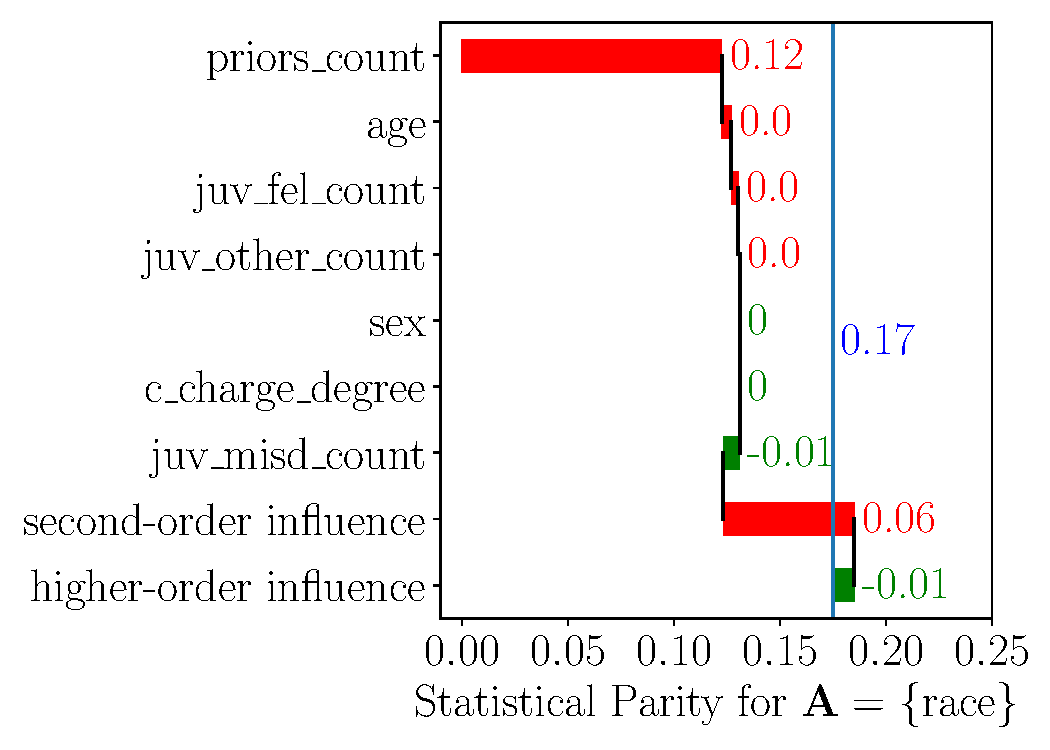
\includegraphics[scale=0.35]{figures/fairness/fif/feature_weight_unsorted}\label{fig:individual_fifs}}
	\end{minipage}
	\begin{minipage}{0.5\textwidth}
		\centering
		\subfloat[Individual and intersectional FIFs]{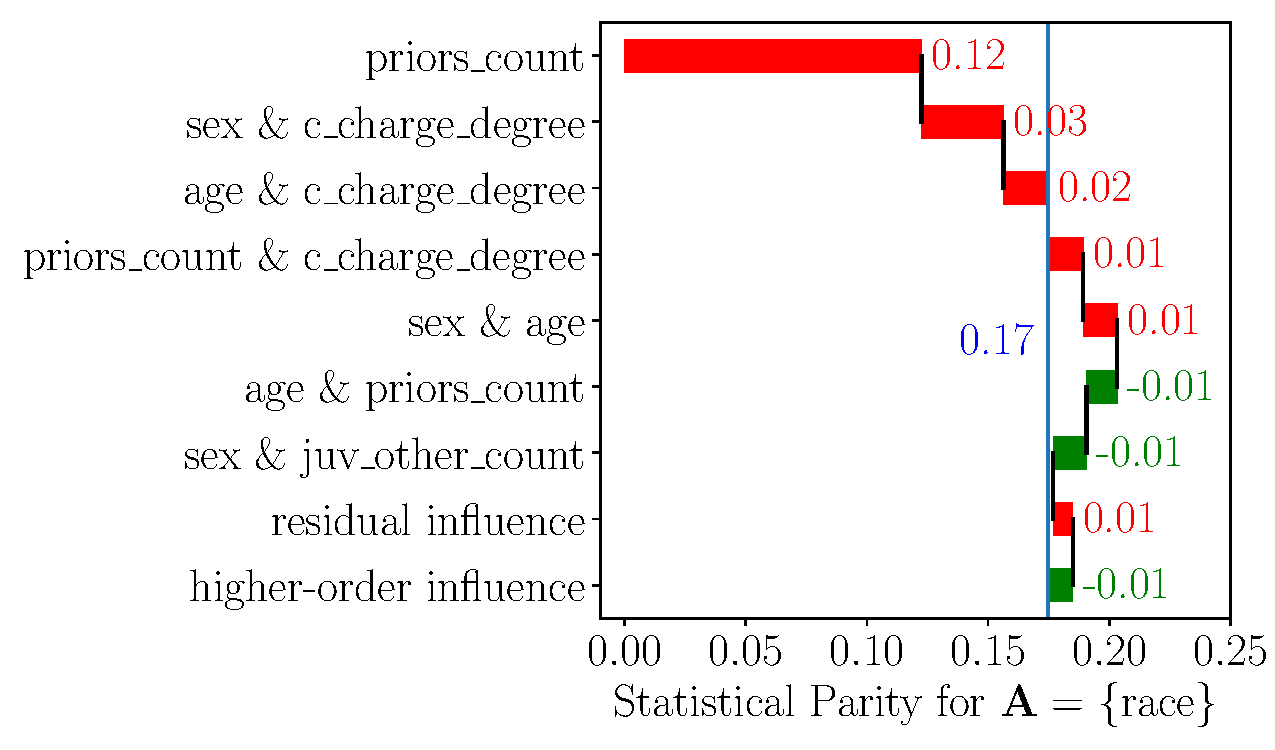
\includegraphics[scale=0.35]{figures/fairness/fif/feature_weight}\label{fig:individual_and_intersectional_fifs}}
	\end{minipage}
	\vspace{-0.2em}
	\caption[Individual vs.\ intersectional FIFs]{FIFs for COMPAS dataset on explaining statistical parity. Intersectional FIFs depict sources of bias in detail than individual FIFs.}\label{fig:individual_vs_intersectional_influence}
	
\end{figure}
\begin{figure}[t!]
	\vspace{-0.7em}
	\begin{minipage}{0.49\textwidth}
		\centering
		\subfloat[Fairness attack (punitive actions)]{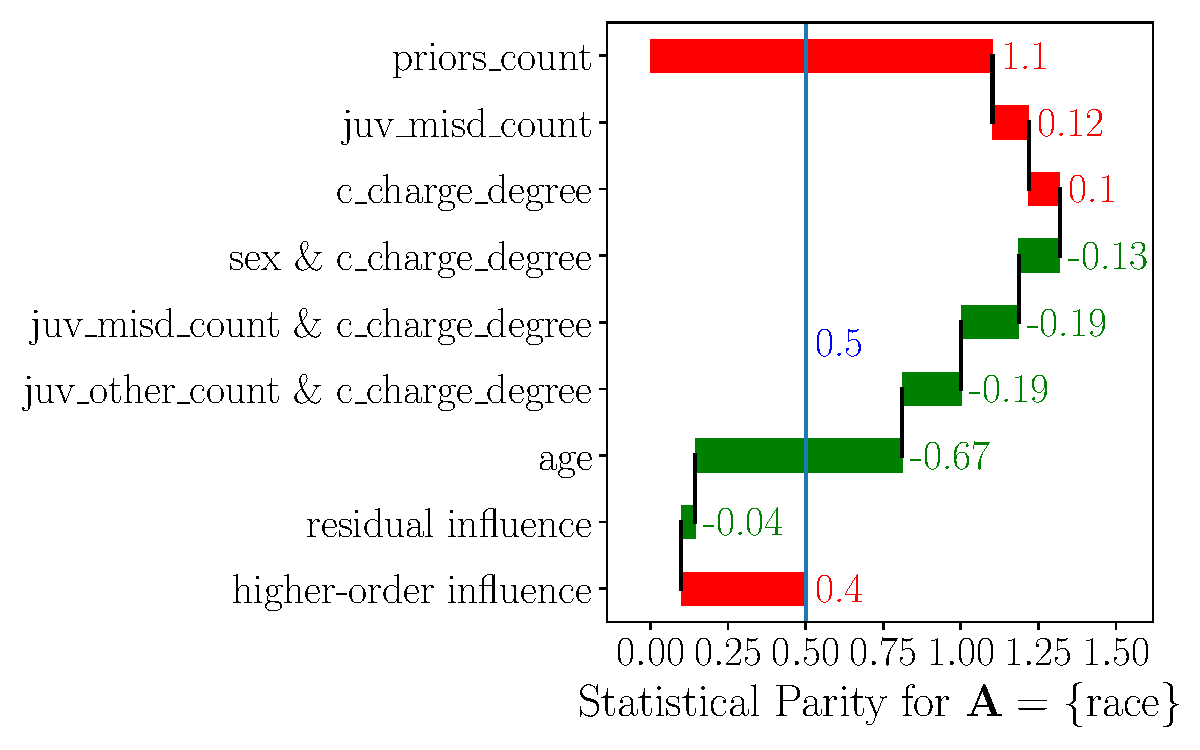
\includegraphics[scale=0.345]{figures/fairness/fif/fairness_attack}\label{fig:fairness_attack}}
	\end{minipage}
	\begin{minipage}{0.5\textwidth}
		\centering	
		\subfloat[Fairness enchancing algorithm (affirmative actions)]{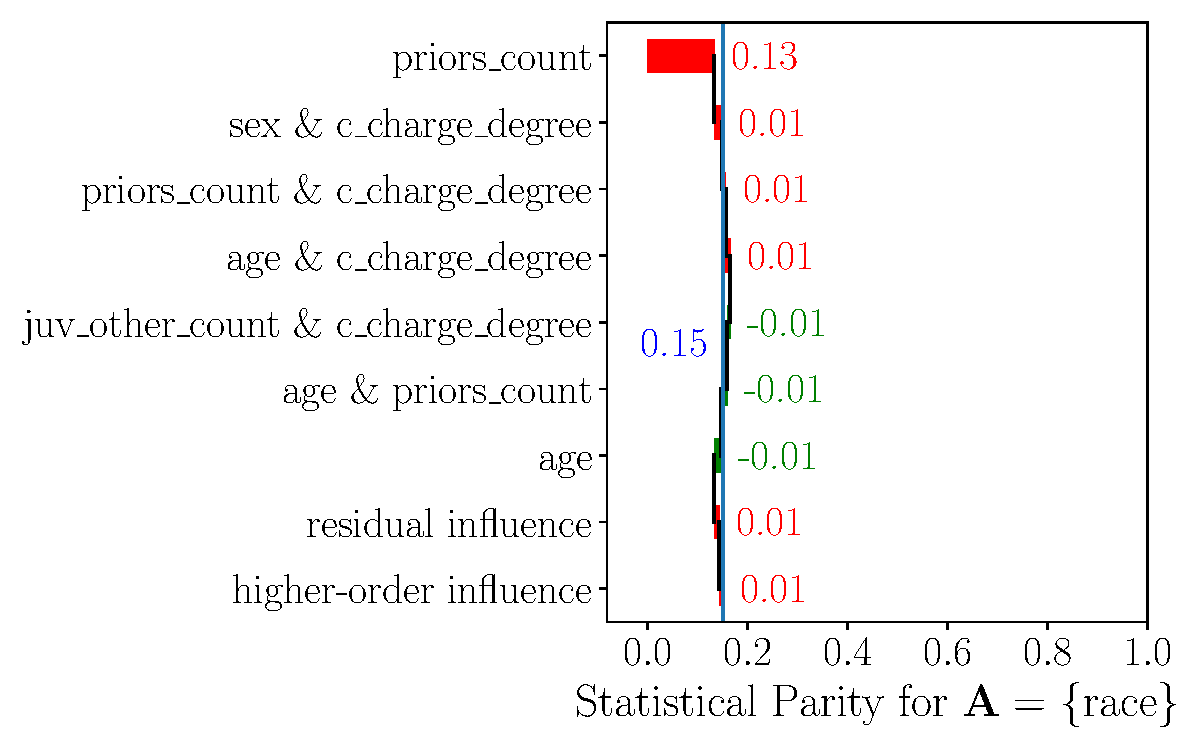
\includegraphics[scale=0.345]{figures/fairness/fif/fairness_repair}\label{fig:fairness_repair}}
	\end{minipage}
	\vspace{-0.2em}
	\caption[FIFs under fairness attack and fairness enhancing algorithms]{Effects of a fairness attack~\cite{solans2020poisoning} and a fairness enhancing algorithm~\cite{kamiran2012data} on FIFs.}\label{fig:affirmative_punitive_actions}
%	\vspace{-0.5em}
\end{figure}

\noindent\textbf{Fairness affirmative/punitive actions.} Continuing on the experiment in Figure~\ref{fig:individual_vs_intersectional_influence}, we evaluate the effect of fairness attack and enhancing algorithms on FIFs for COMPAS dataset in Figure~\ref{fig:affirmative_punitive_actions}.  In Figure~\ref{fig:individual_vs_intersectional_influence}, statistical parity of the classifier is $ 0.17 $. Applying a data poisoning fairness attack~\cite{solans2020poisoning} increases statistical parity to $ 0.5 $ and the data reweighing-based fairness-enhancing algorithm~\cite{kamiran2012data} decreases it to $ 0.15$. We observe that in both cases, there are a subset of features decreasing bias while another subset of features increasing it, e.g. `age' vs.\ `priors count'. Figure~\ref{fig:fairness_attack} suggests that the attack algorithm would be more successful if it could hide the influence of `age' of a person in receiving discriminating prediction for re-offending crimes. Figure~\ref{fig:fairness_repair} suggests that the fairness enhancing algorithm can improve by ameliorating the effect of `priors count' further. Thus, \textit{{\fairXplainer} provides a dissecting tool to undertake necessary steps to improve or worsen fairness of the classifier.}



